\documentclass{article}
\usepackage{graphicx}
\usepackage{float}

\title{Laboratory Work 9 Report: Nonlinear Dimension Reduction}
\author{Your Name}

\begin{document}

\maketitle

\section{Introduction}
In this laboratory work, the focus was on applying various nonlinear dimension reduction techniques and evaluating their effectiveness in clustering analysis. The methods used include PCA, TruncatedSVD, Factor Analysis, t-SNE, MDS, and Kernel PCA. The primary objective was to reduce the dimensionality of the data while preserving meaningful relationships among data points for clustering purposes.

\section{Results}

\subsection{Inertia for 2D}

\begin{table}[H]
    \centering
    \begin{tabular}{|l|l|}
    \hline
    \textbf{Method} & \textbf{Inertia} \\ \hline
    PCA & 406.16 \\ \hline
    TruncatedSVD & 406.16 \\ \hline
    Factor Analysis & 176.48 \\ \hline
    t-SNE & 12287.63 \\ \hline
    MDS & 751.34 \\ \hline
    Kernel PCA & 406.16 \\ \hline
    \end{tabular}
    \caption{Inertia values for 2D dimensionality reduction methods}
    \label{tab:inertia_2d}
\end{table}

\subsubsection{Comments}
\begin{itemize}
    \item \textbf{PCA, TruncatedSVD, Kernel PCA}: These methods exhibit similar inertia values, suggesting comparable clustering results in 2D space.
    \item \textbf{Factor Analysis}: Lower inertia indicates more compact clusters compared to linear methods.
    \item \textbf{t-SNE}: Highest inertia indicates more dispersed clusters, typical of its nonlinear nature.
    \item \textbf{MDS}: Moderate inertia implies moderate clustering quality.
\end{itemize}

\begin{figure}[H]
    \centering
    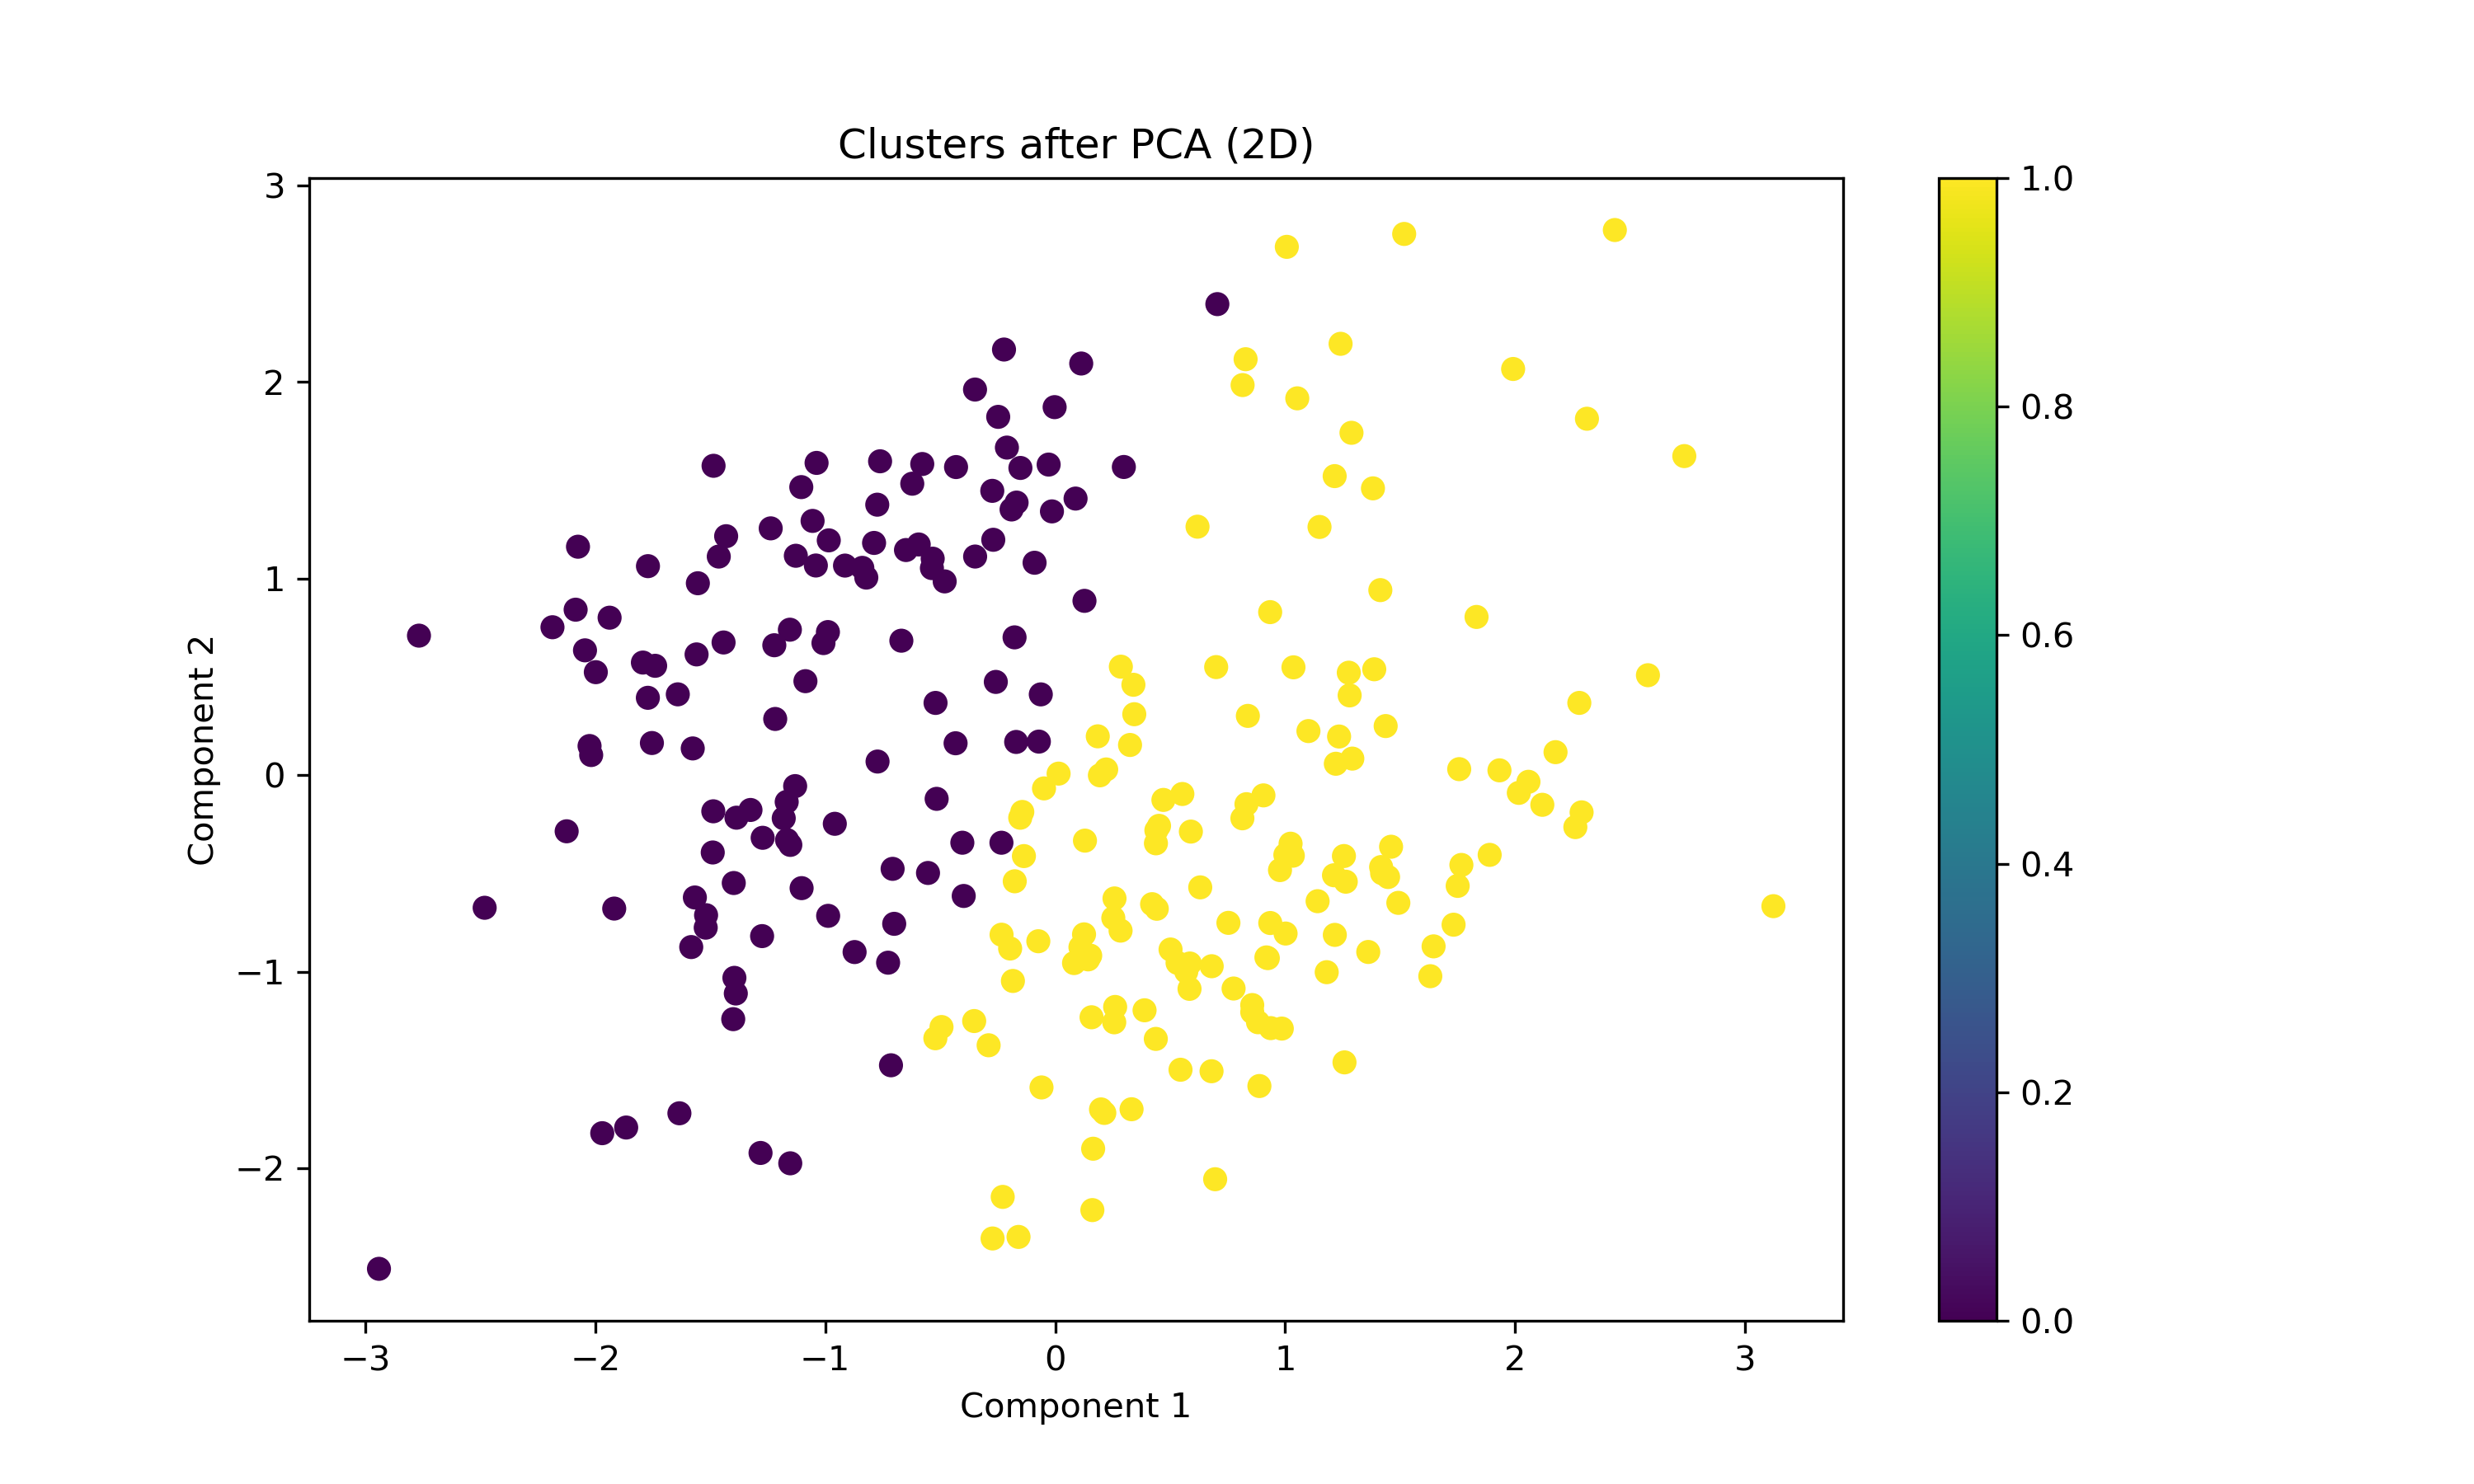
\includegraphics[width=0.5\linewidth]{PCA_2D.png}
    \caption{Clusters after PCA (2D)}
    \label{fig:pca_2d}
\end{figure}

\begin{figure}[H]
    \centering
    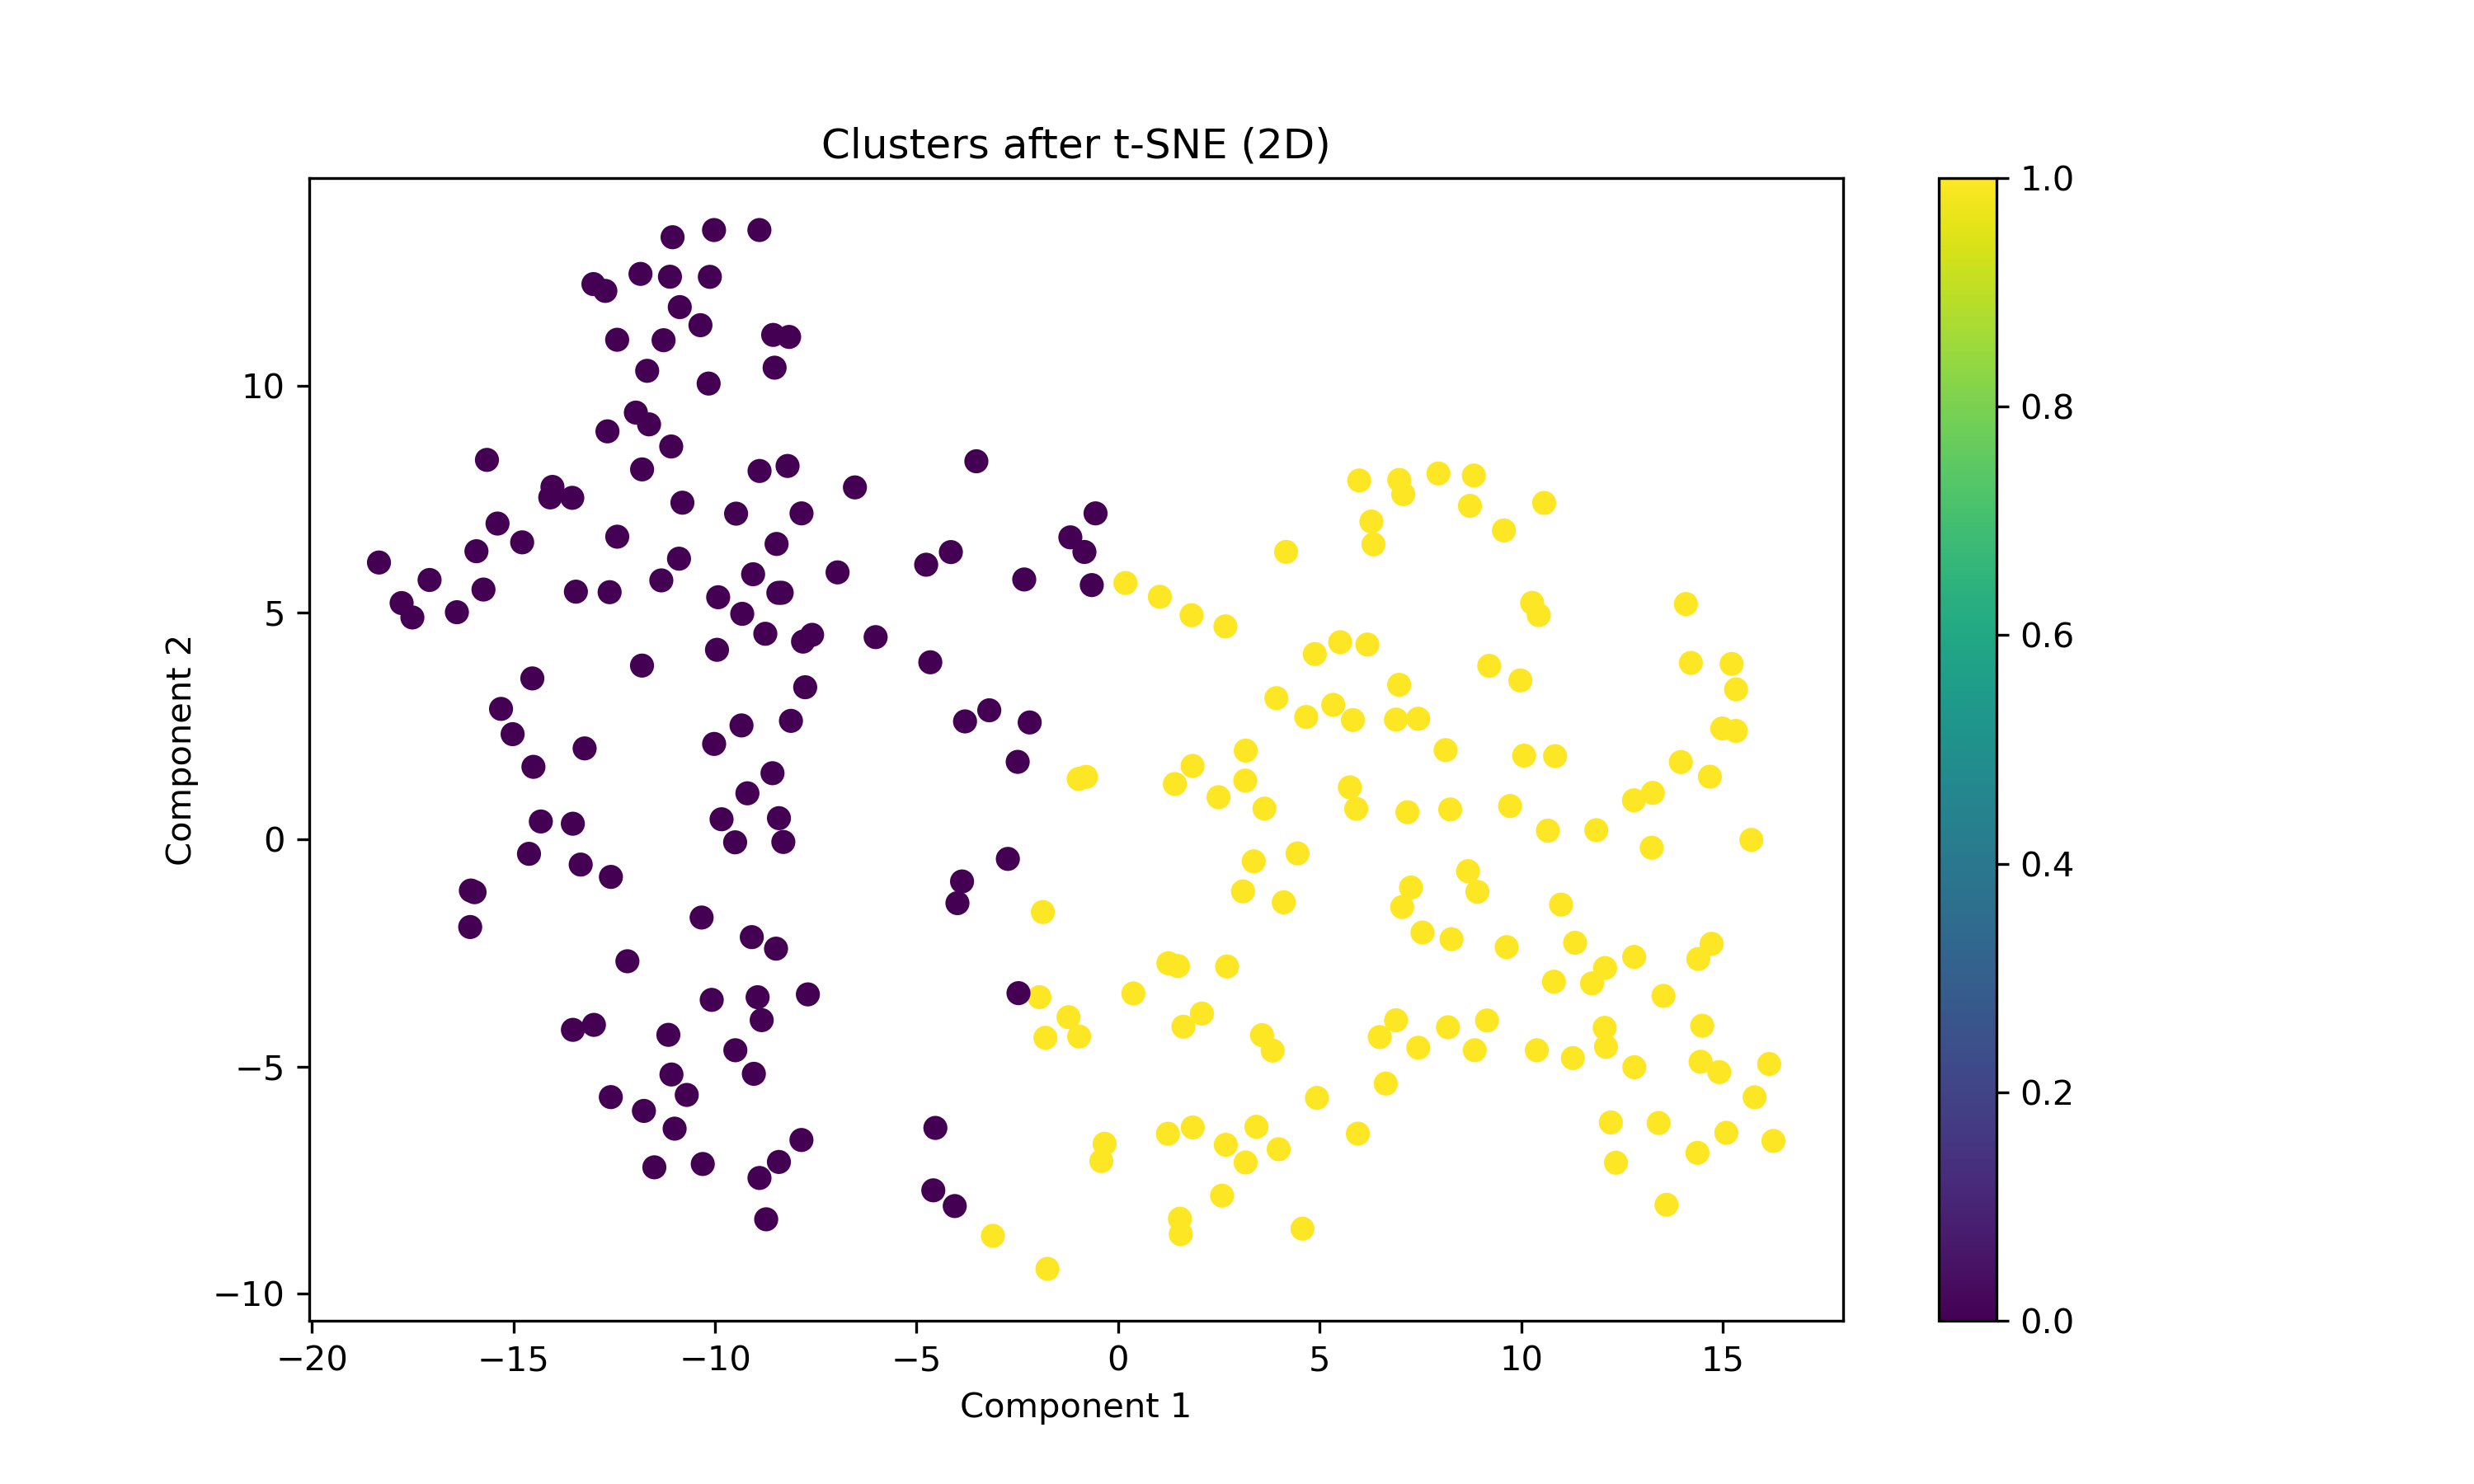
\includegraphics[width=0.5\linewidth]{t-SNE_2D.png}
    \caption{Clusters after t-SNE (2D)}
    \label{fig:tsne_2d}
\end{figure}

\begin{figure}[H]
    \centering
    \includegraphics[width=0.5\linewidth]{Kernel_PCA_2D.png}
    \caption{Clusters after Kernel PCA (2D)}
    \label{fig:kernel_pca_2d}
\end{figure}

\begin{figure}[H]
    \centering
    \includegraphics[width=0.5\linewidth]{Factor_Analysis_2D.png}
    \caption{Clusters after Factor Analysis (2D)}
    \label{fig:factor_analysis_2d}
\end{figure}

\begin{figure}[H]
    \centering
    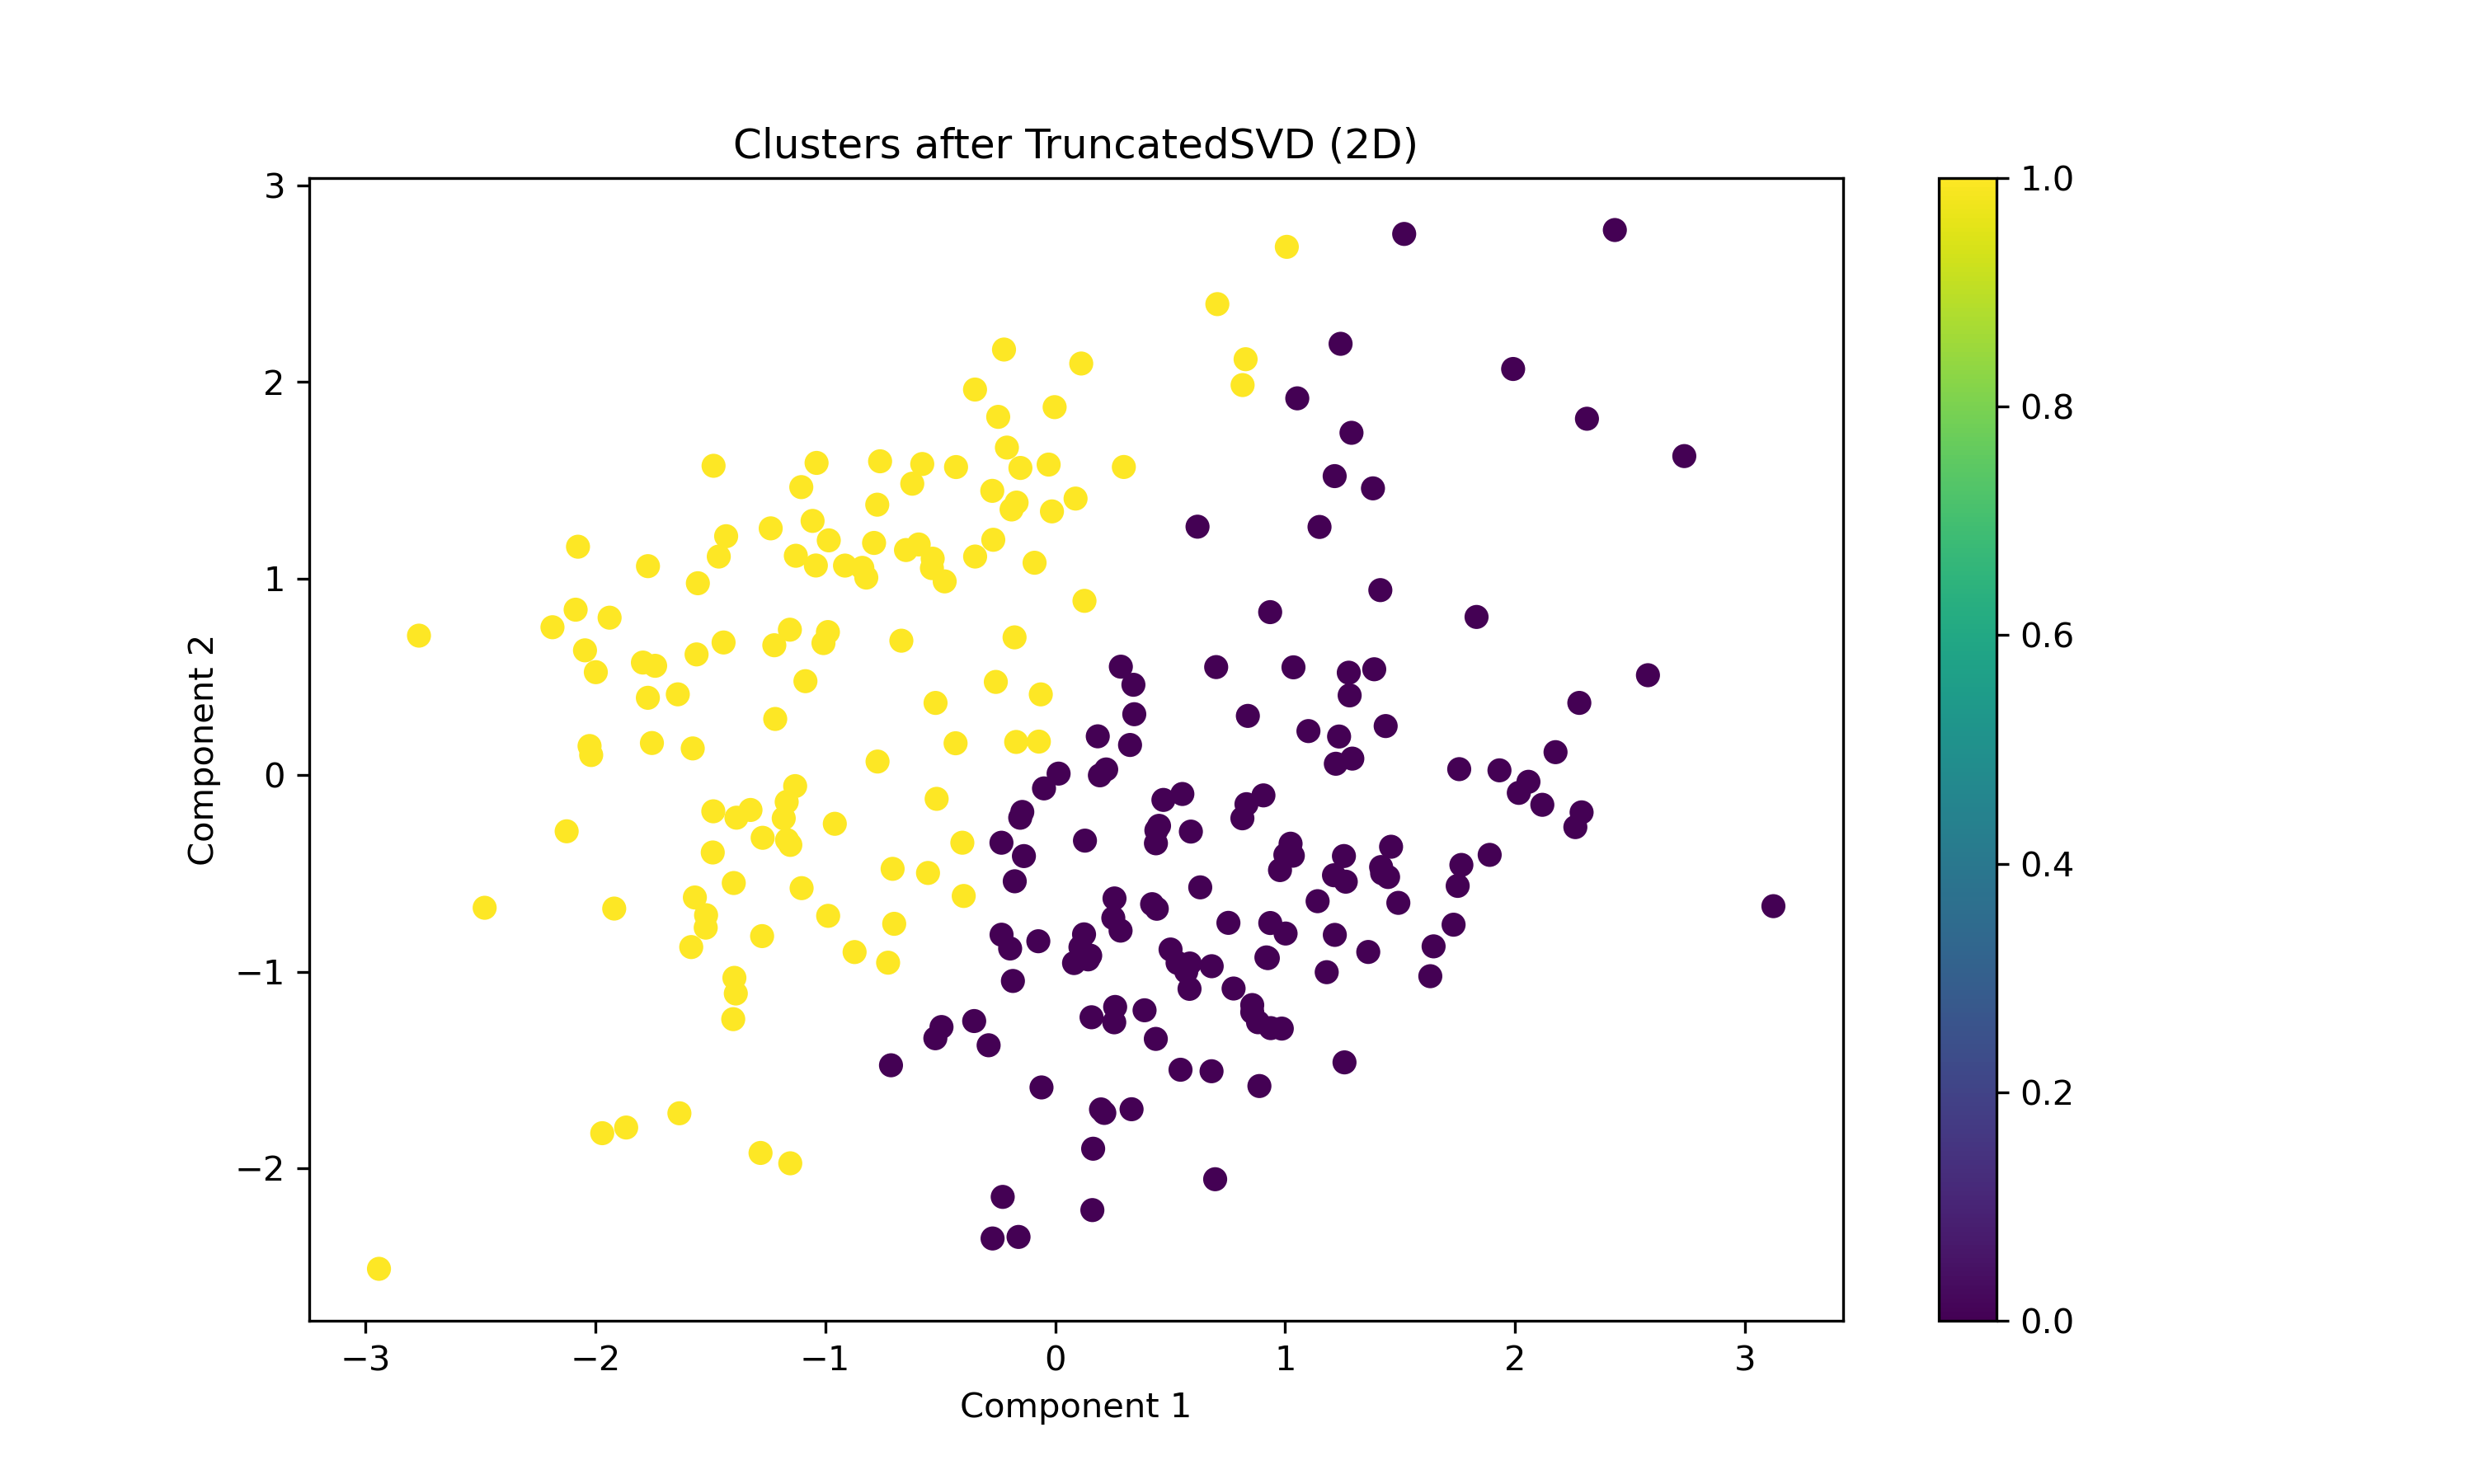
\includegraphics[width=0.5\linewidth]{TruncatedSVD_2D.png}
    \caption{Clusters after TruncatedSVD (2D)}
    \label{fig:truncated_svd_2d}
\end{figure}

\begin{figure}[H]
    \centering
    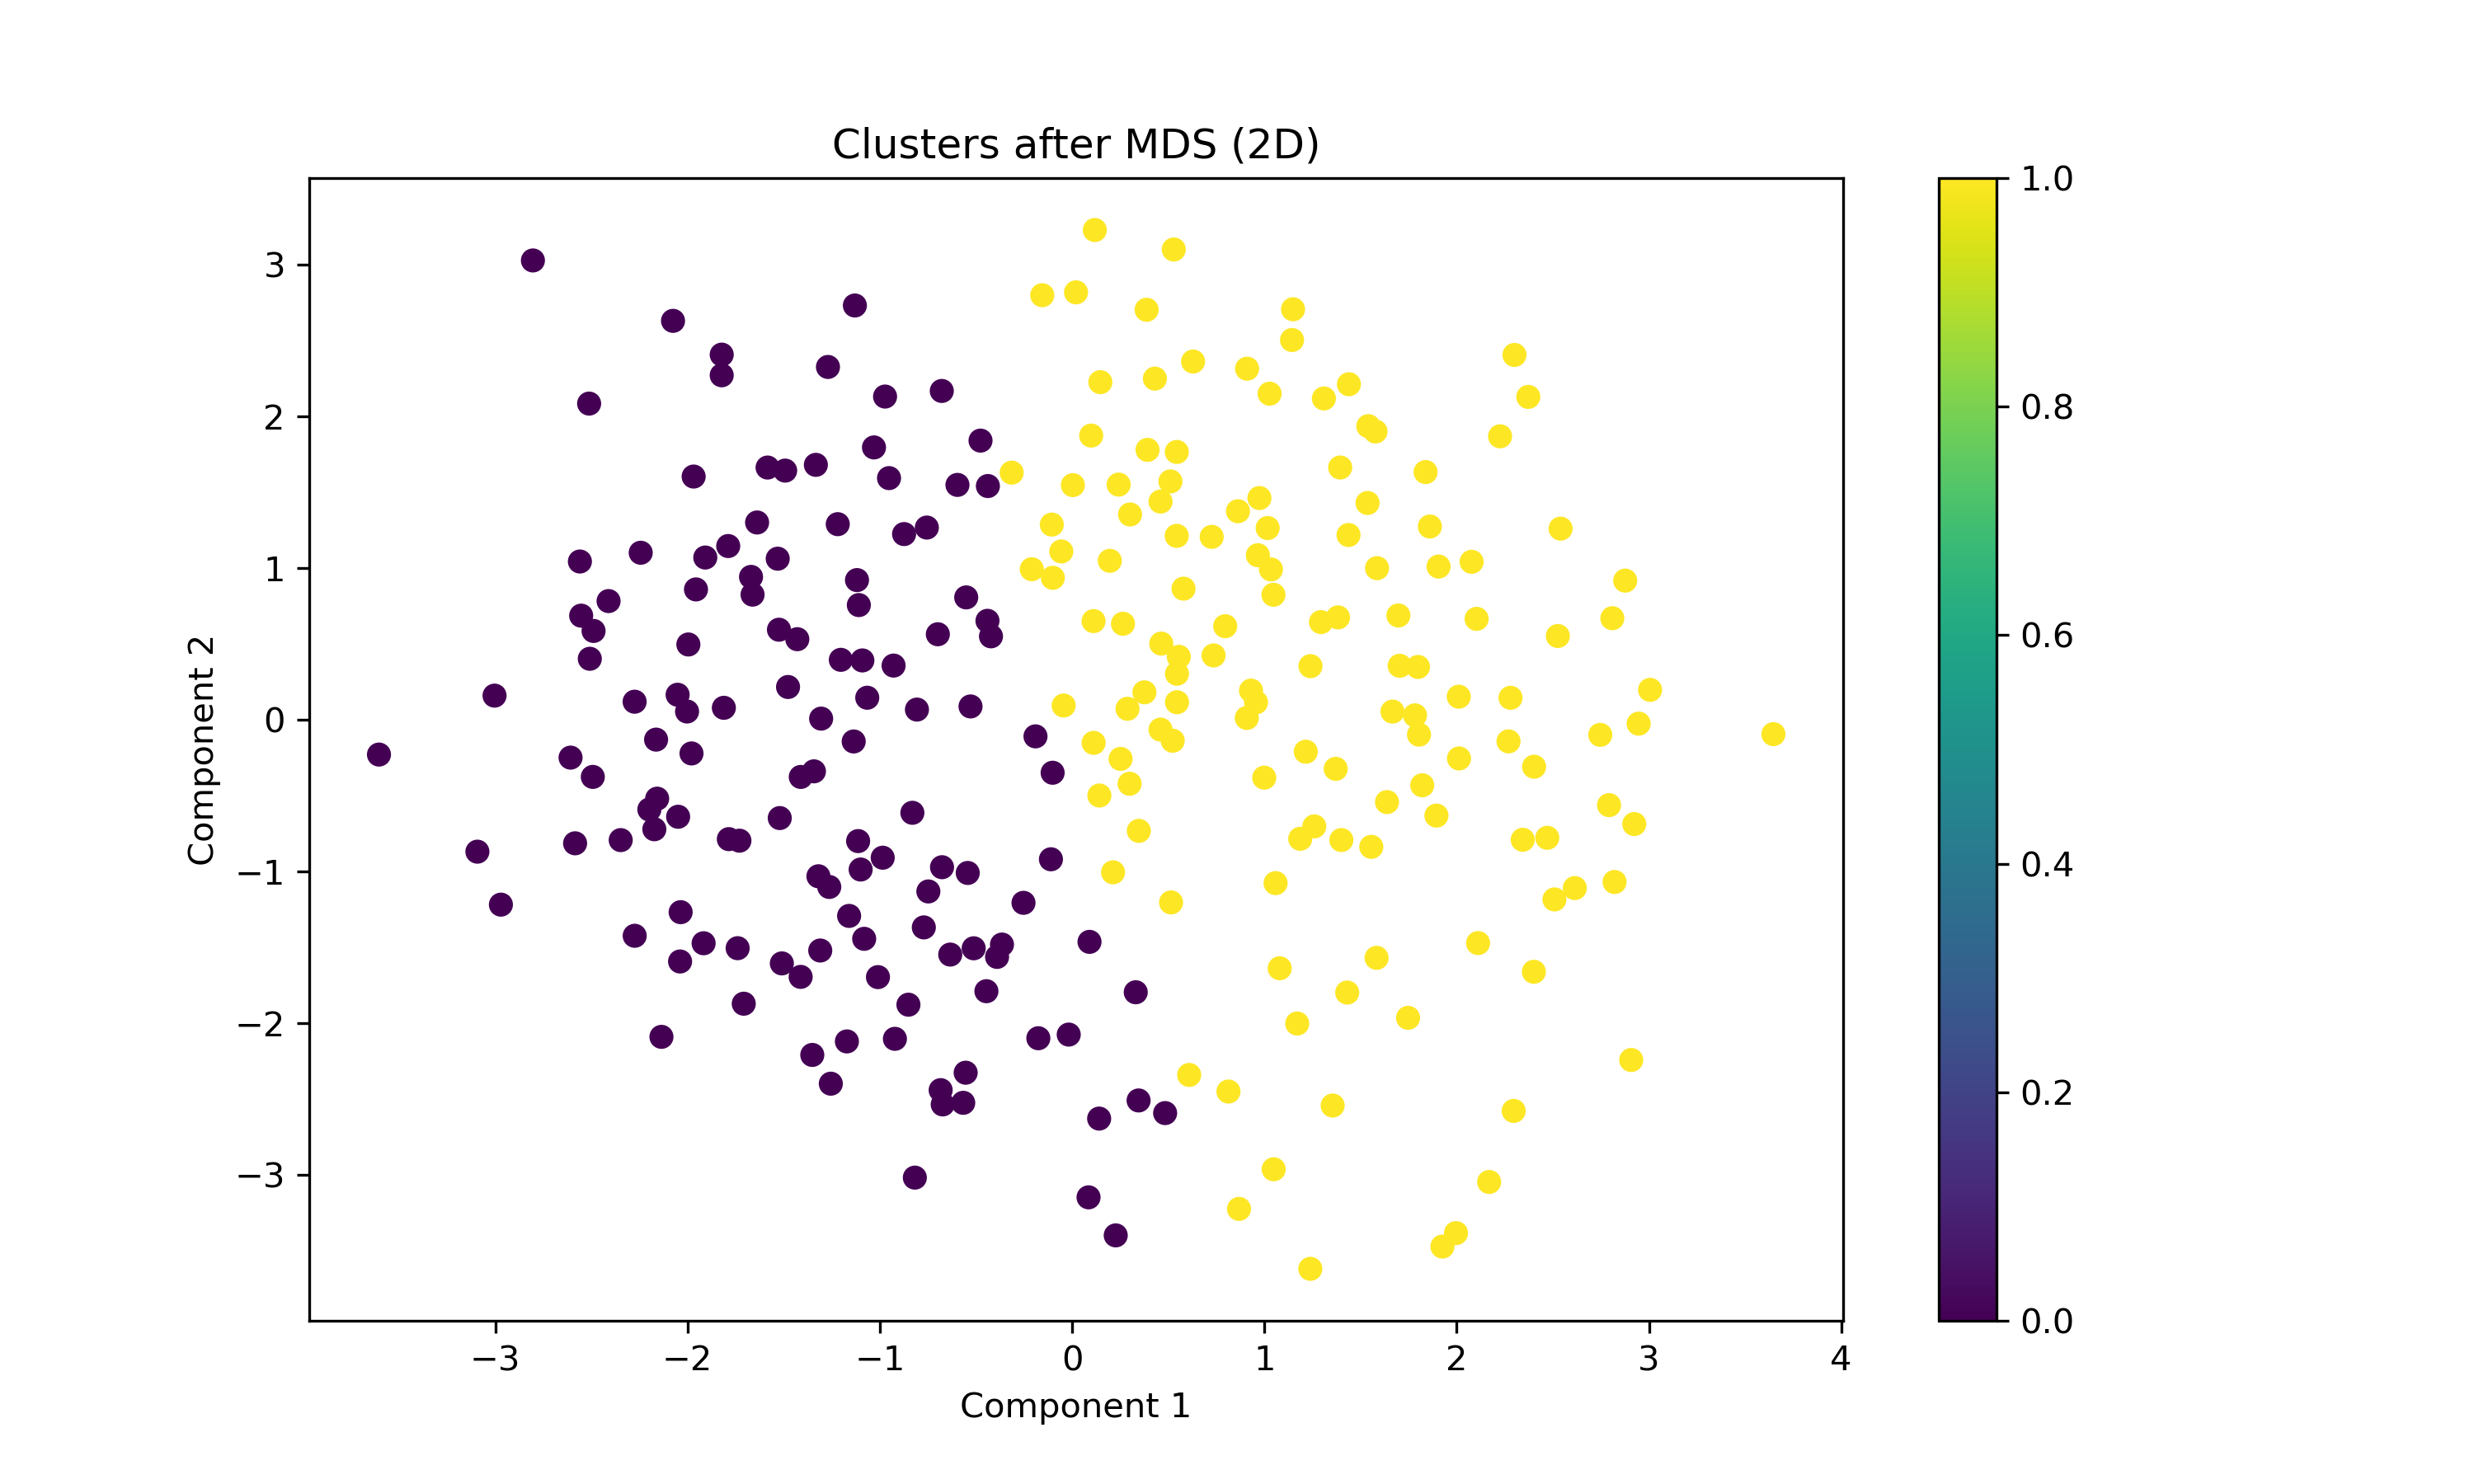
\includegraphics[width=0.5\linewidth]{MDS_2D.png}
    \caption{Clusters after MDS (2D)}
    \label{fig:mds_2d}
\end{figure}

\subsection{Inertia for 3D}

\begin{table}[H]
    \centering
    \begin{tabular}{|l|l|}
    \hline
    \textbf{Method} & \textbf{Inertia} \\ \hline
    PCA & 655.58 \\ \hline
    TruncatedSVD & 655.58 \\ \hline
    Factor Analysis & 220.71 \\ \hline
    t-SNE & 3761.99 \\ \hline
    MDS & 946.10 \\ \hline
    Kernel PCA & 655.58 \\ \hline
    \end{tabular}
    \caption{Inertia values for 3D dimensionality reduction methods}
    \label{tab:inertia_3d}
\end{table}

\subsubsection{Comments}
\begin{itemize}
    \item \textbf{PCA, TruncatedSVD, Kernel PCA}: Consistent inertia values across methods indicate stable clustering in 3D.
    \item \textbf{Factor Analysis}: Lower inertia suggests better clustering than PCA and TruncatedSVD.
    \item \textbf{t-SNE}: Highest inertia indicates more scattered clusters, typical of its nonlinear mapping.
    \item \textbf{MDS}: Moderate inertia indicates moderate clustering performance.
\end{itemize}

\begin{figure}[H]
    \centering
    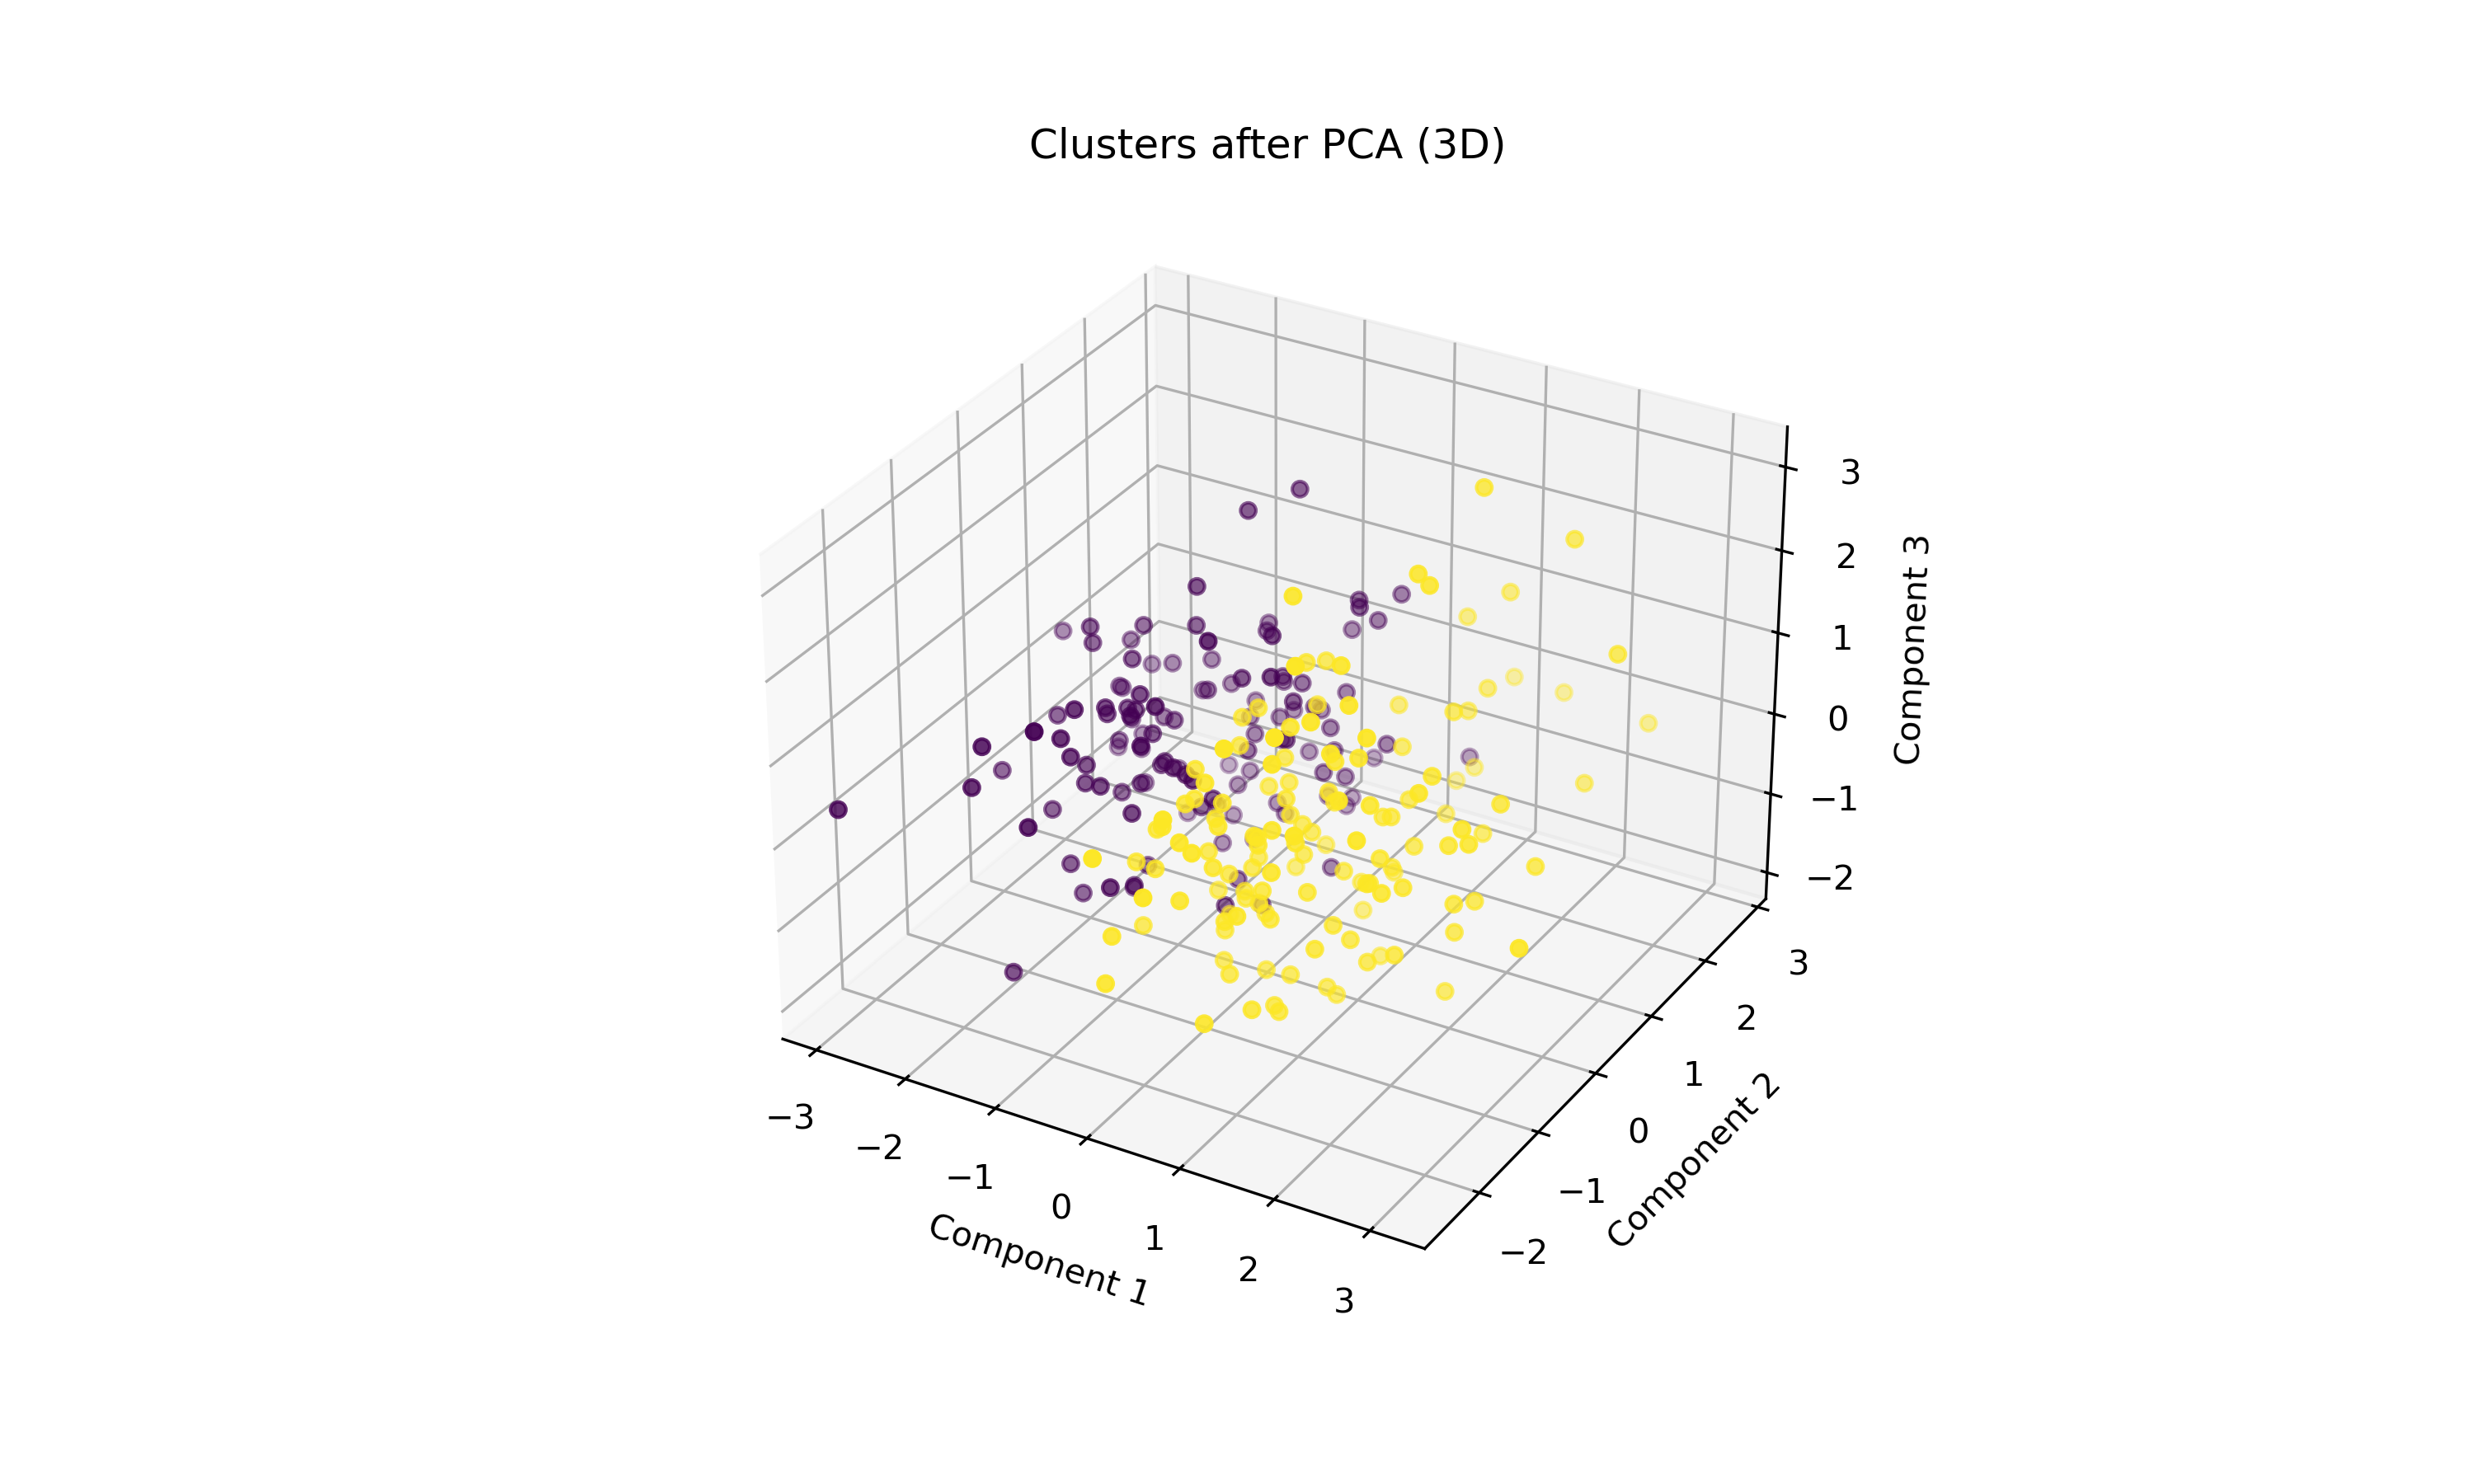
\includegraphics[width=0.5\linewidth]{PCA_3D.png}
    \caption{Clusters after PCA (3D)}
    \label{fig:pca_3d}
\end{figure}

\begin{figure}[H]
    \centering
    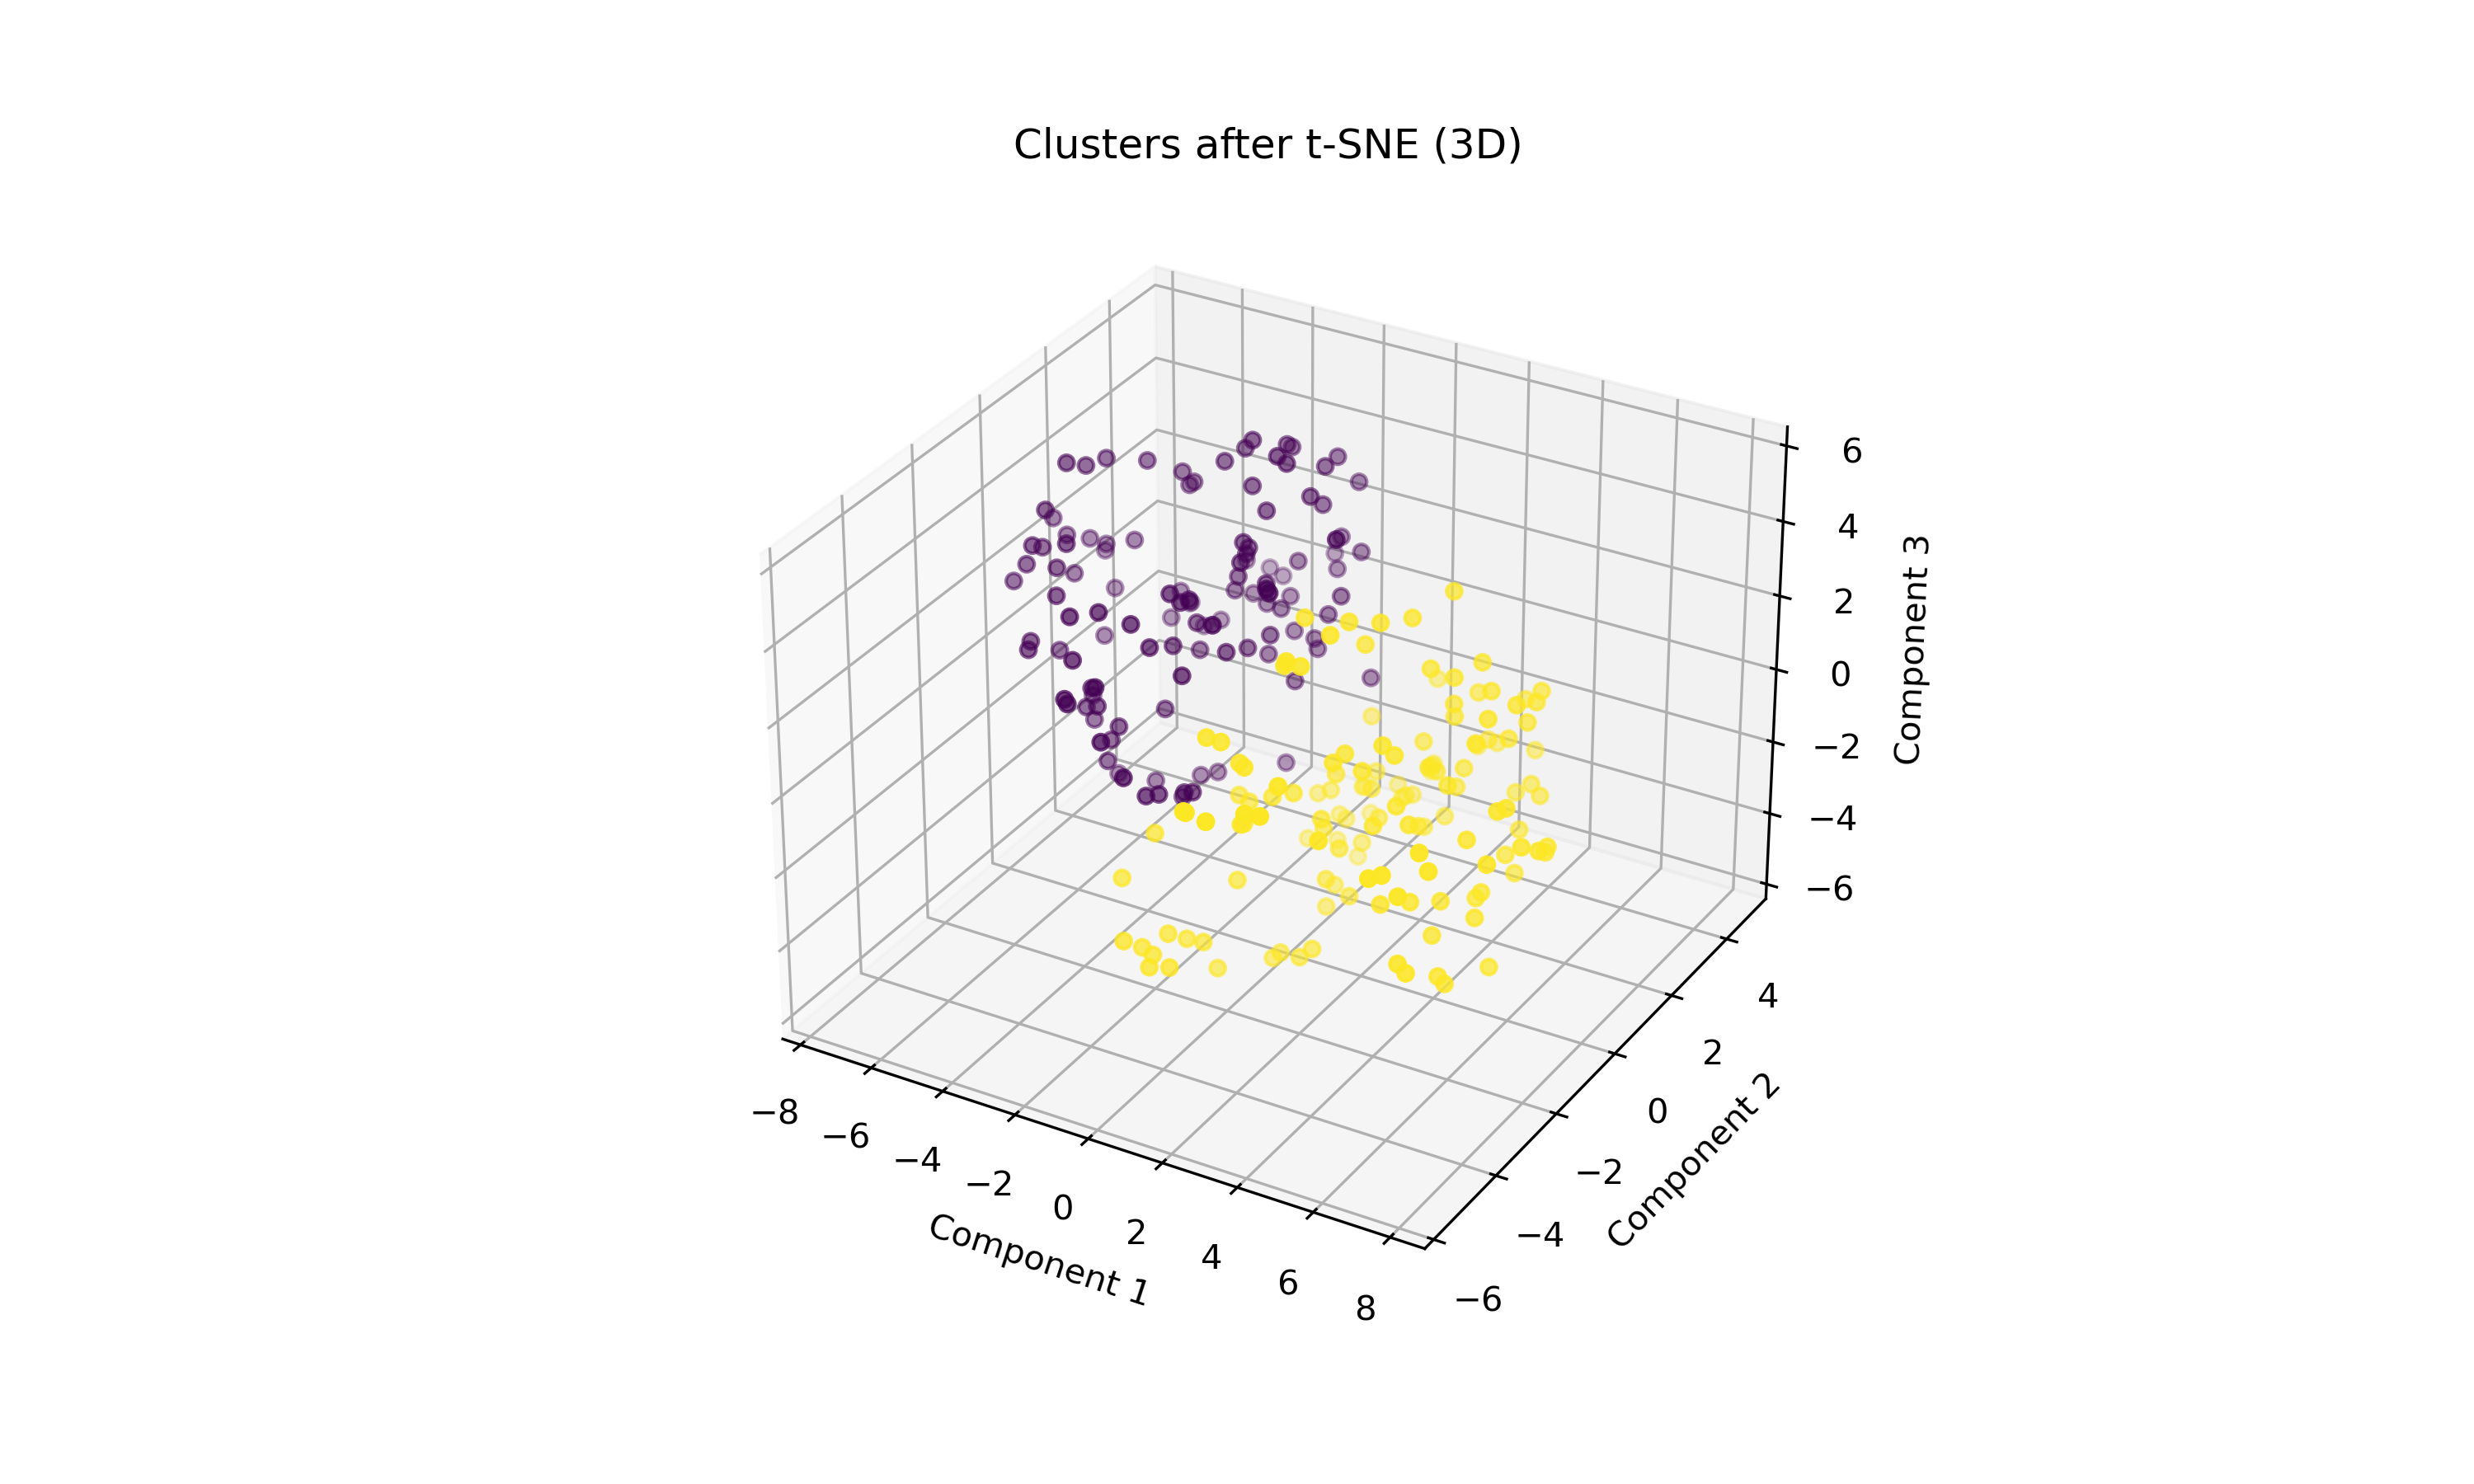
\includegraphics[width=0.5\linewidth]{t-SNE_3D.png}
    \caption{Clusters after t-SNE (3D)}
    \label{fig:tsne_3d}
\end{figure}

\begin{figure}[H]
    \centering
    \includegraphics[width=0.5\linewidth]{Kernel_PCA_3D.png}
    \caption{Clusters after Kernel PCA (3D)}
    \label{fig:kernel_pca_3d}
\end{figure}

\begin{figure}[H]
    \centering
    \includegraphics[width=0.5\linewidth]{Factor_Analysis_3D.png}
    \caption{Clusters after Factor Analysis (3D)}
    \label{fig:factor_analysis_3d}
\end{figure}

\begin{figure}[H]
    \centering
    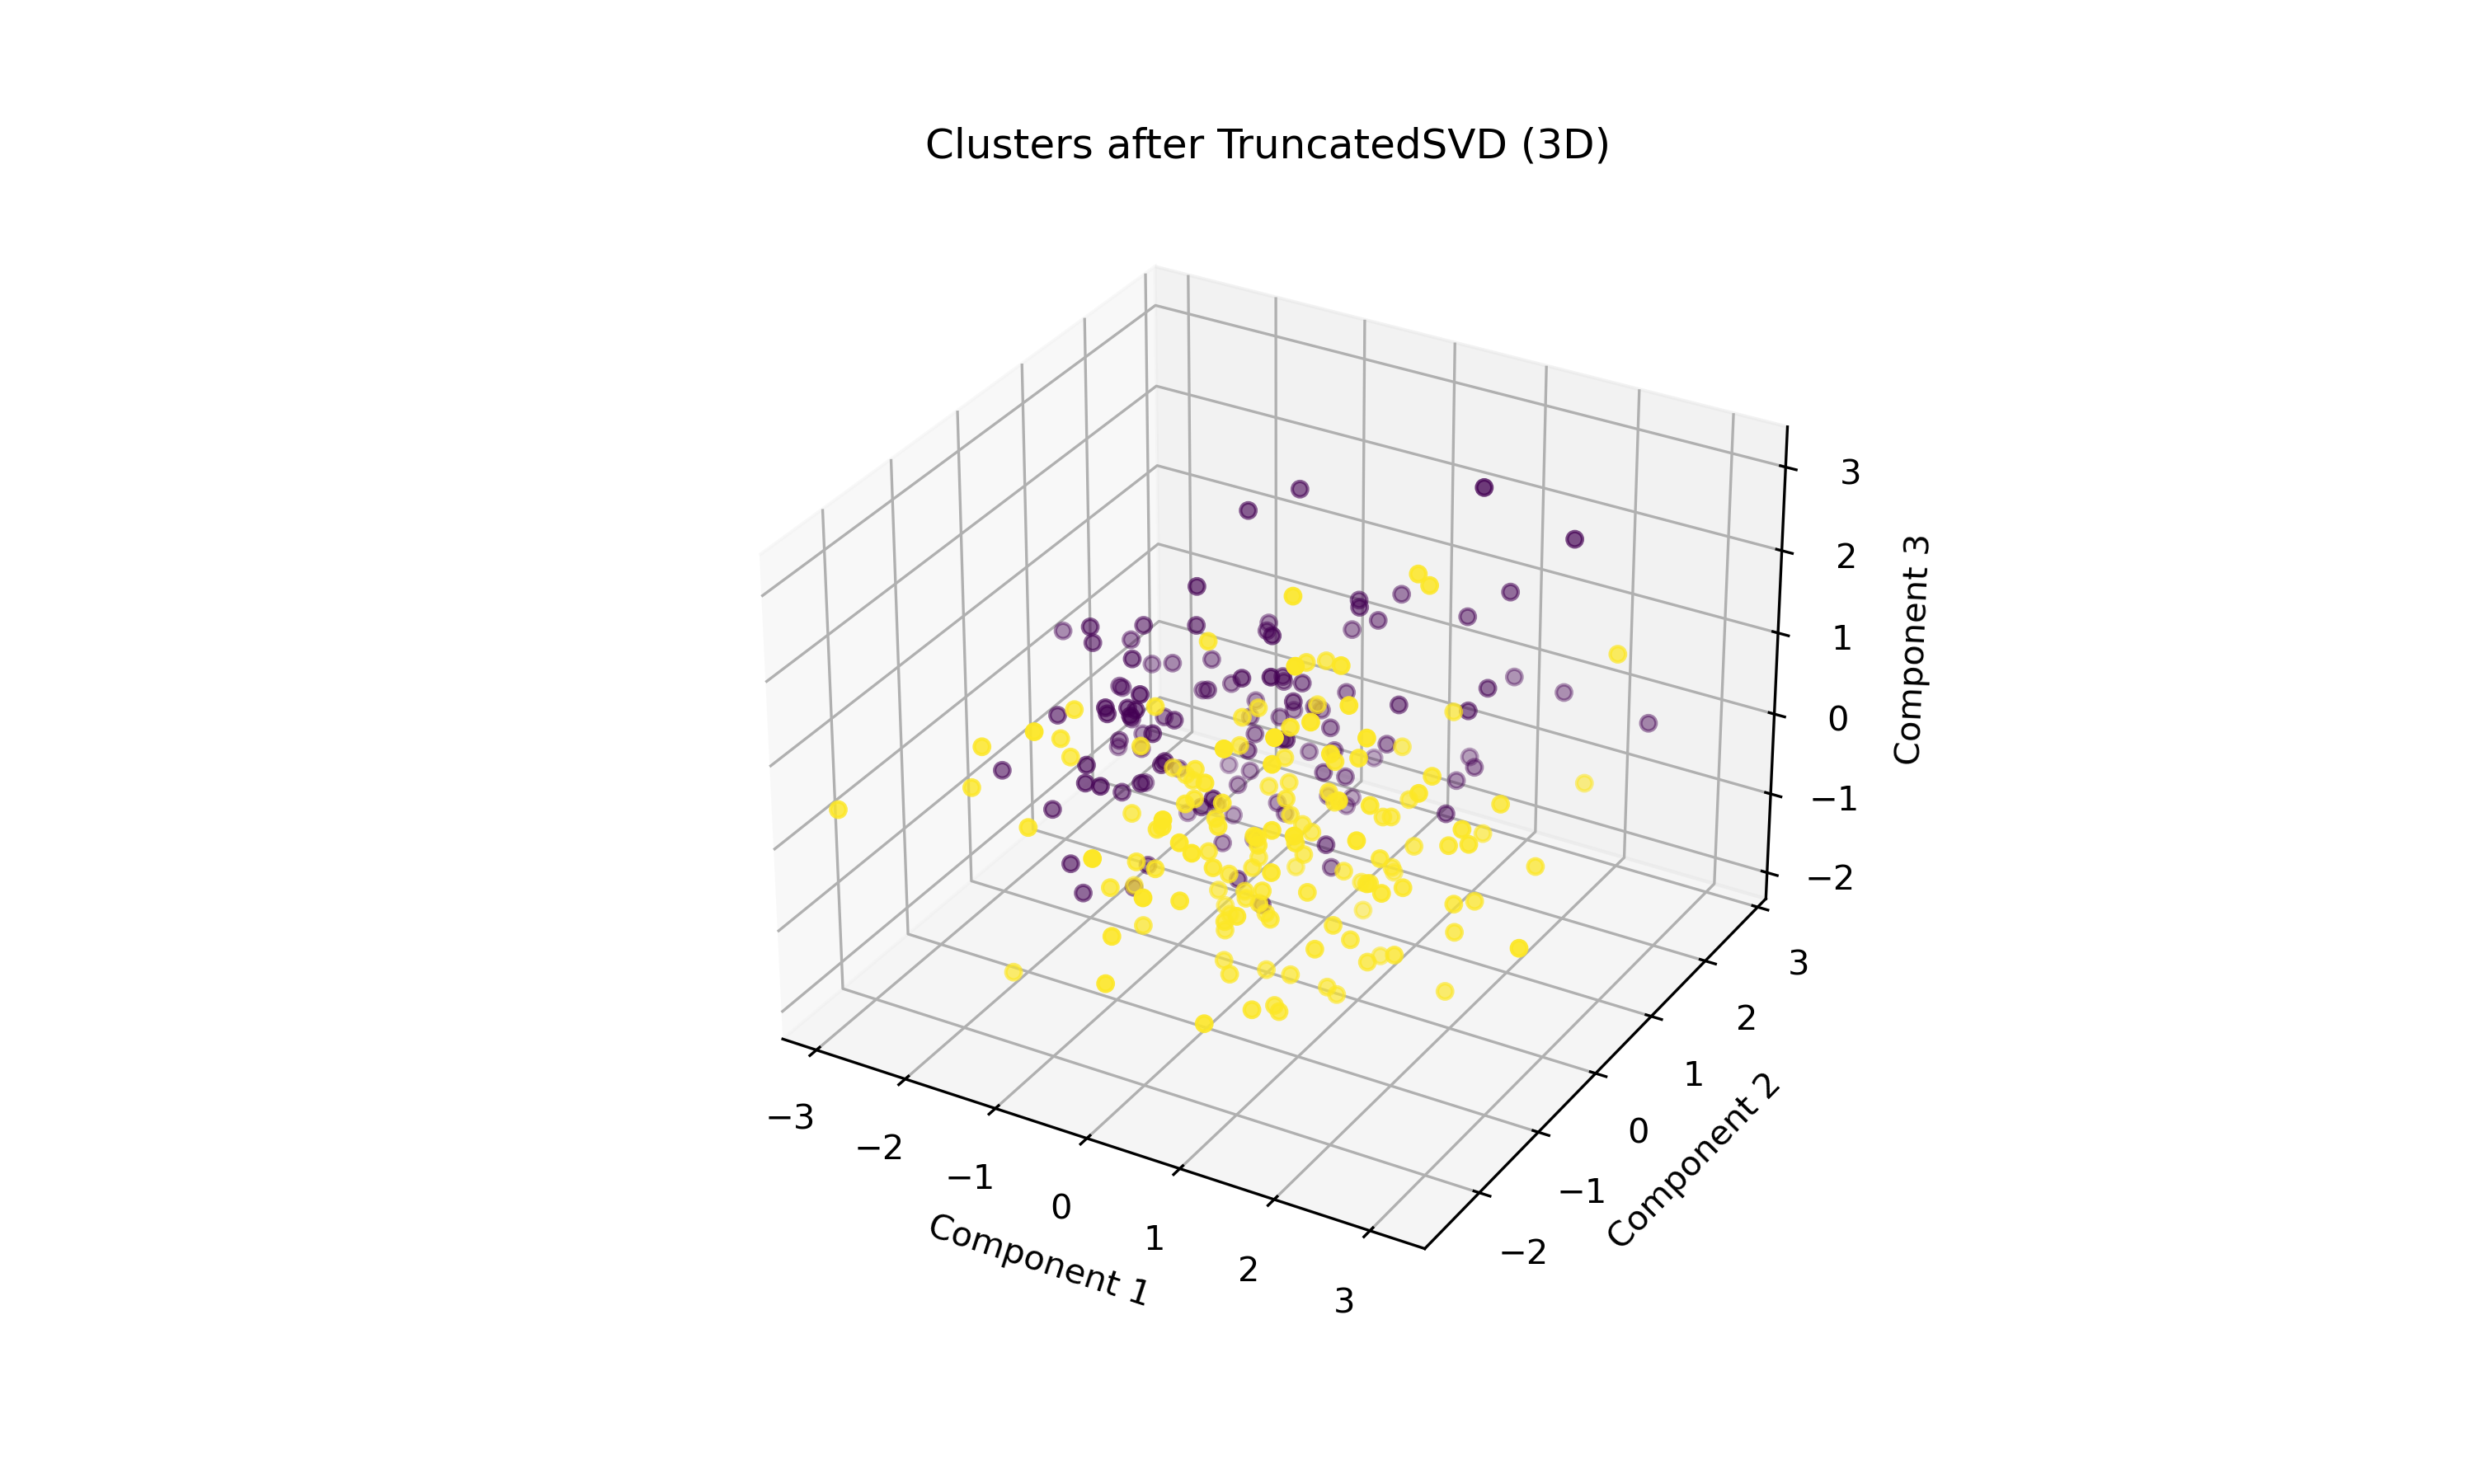
\includegraphics[width=0.5\linewidth]{TruncatedSVD_3D.png}
    \caption{Clusters after TruncatedSVD (3D)}
    \label{fig:truncated_svd_3d}
\end{figure}

\begin{figure}[H]
    \centering
    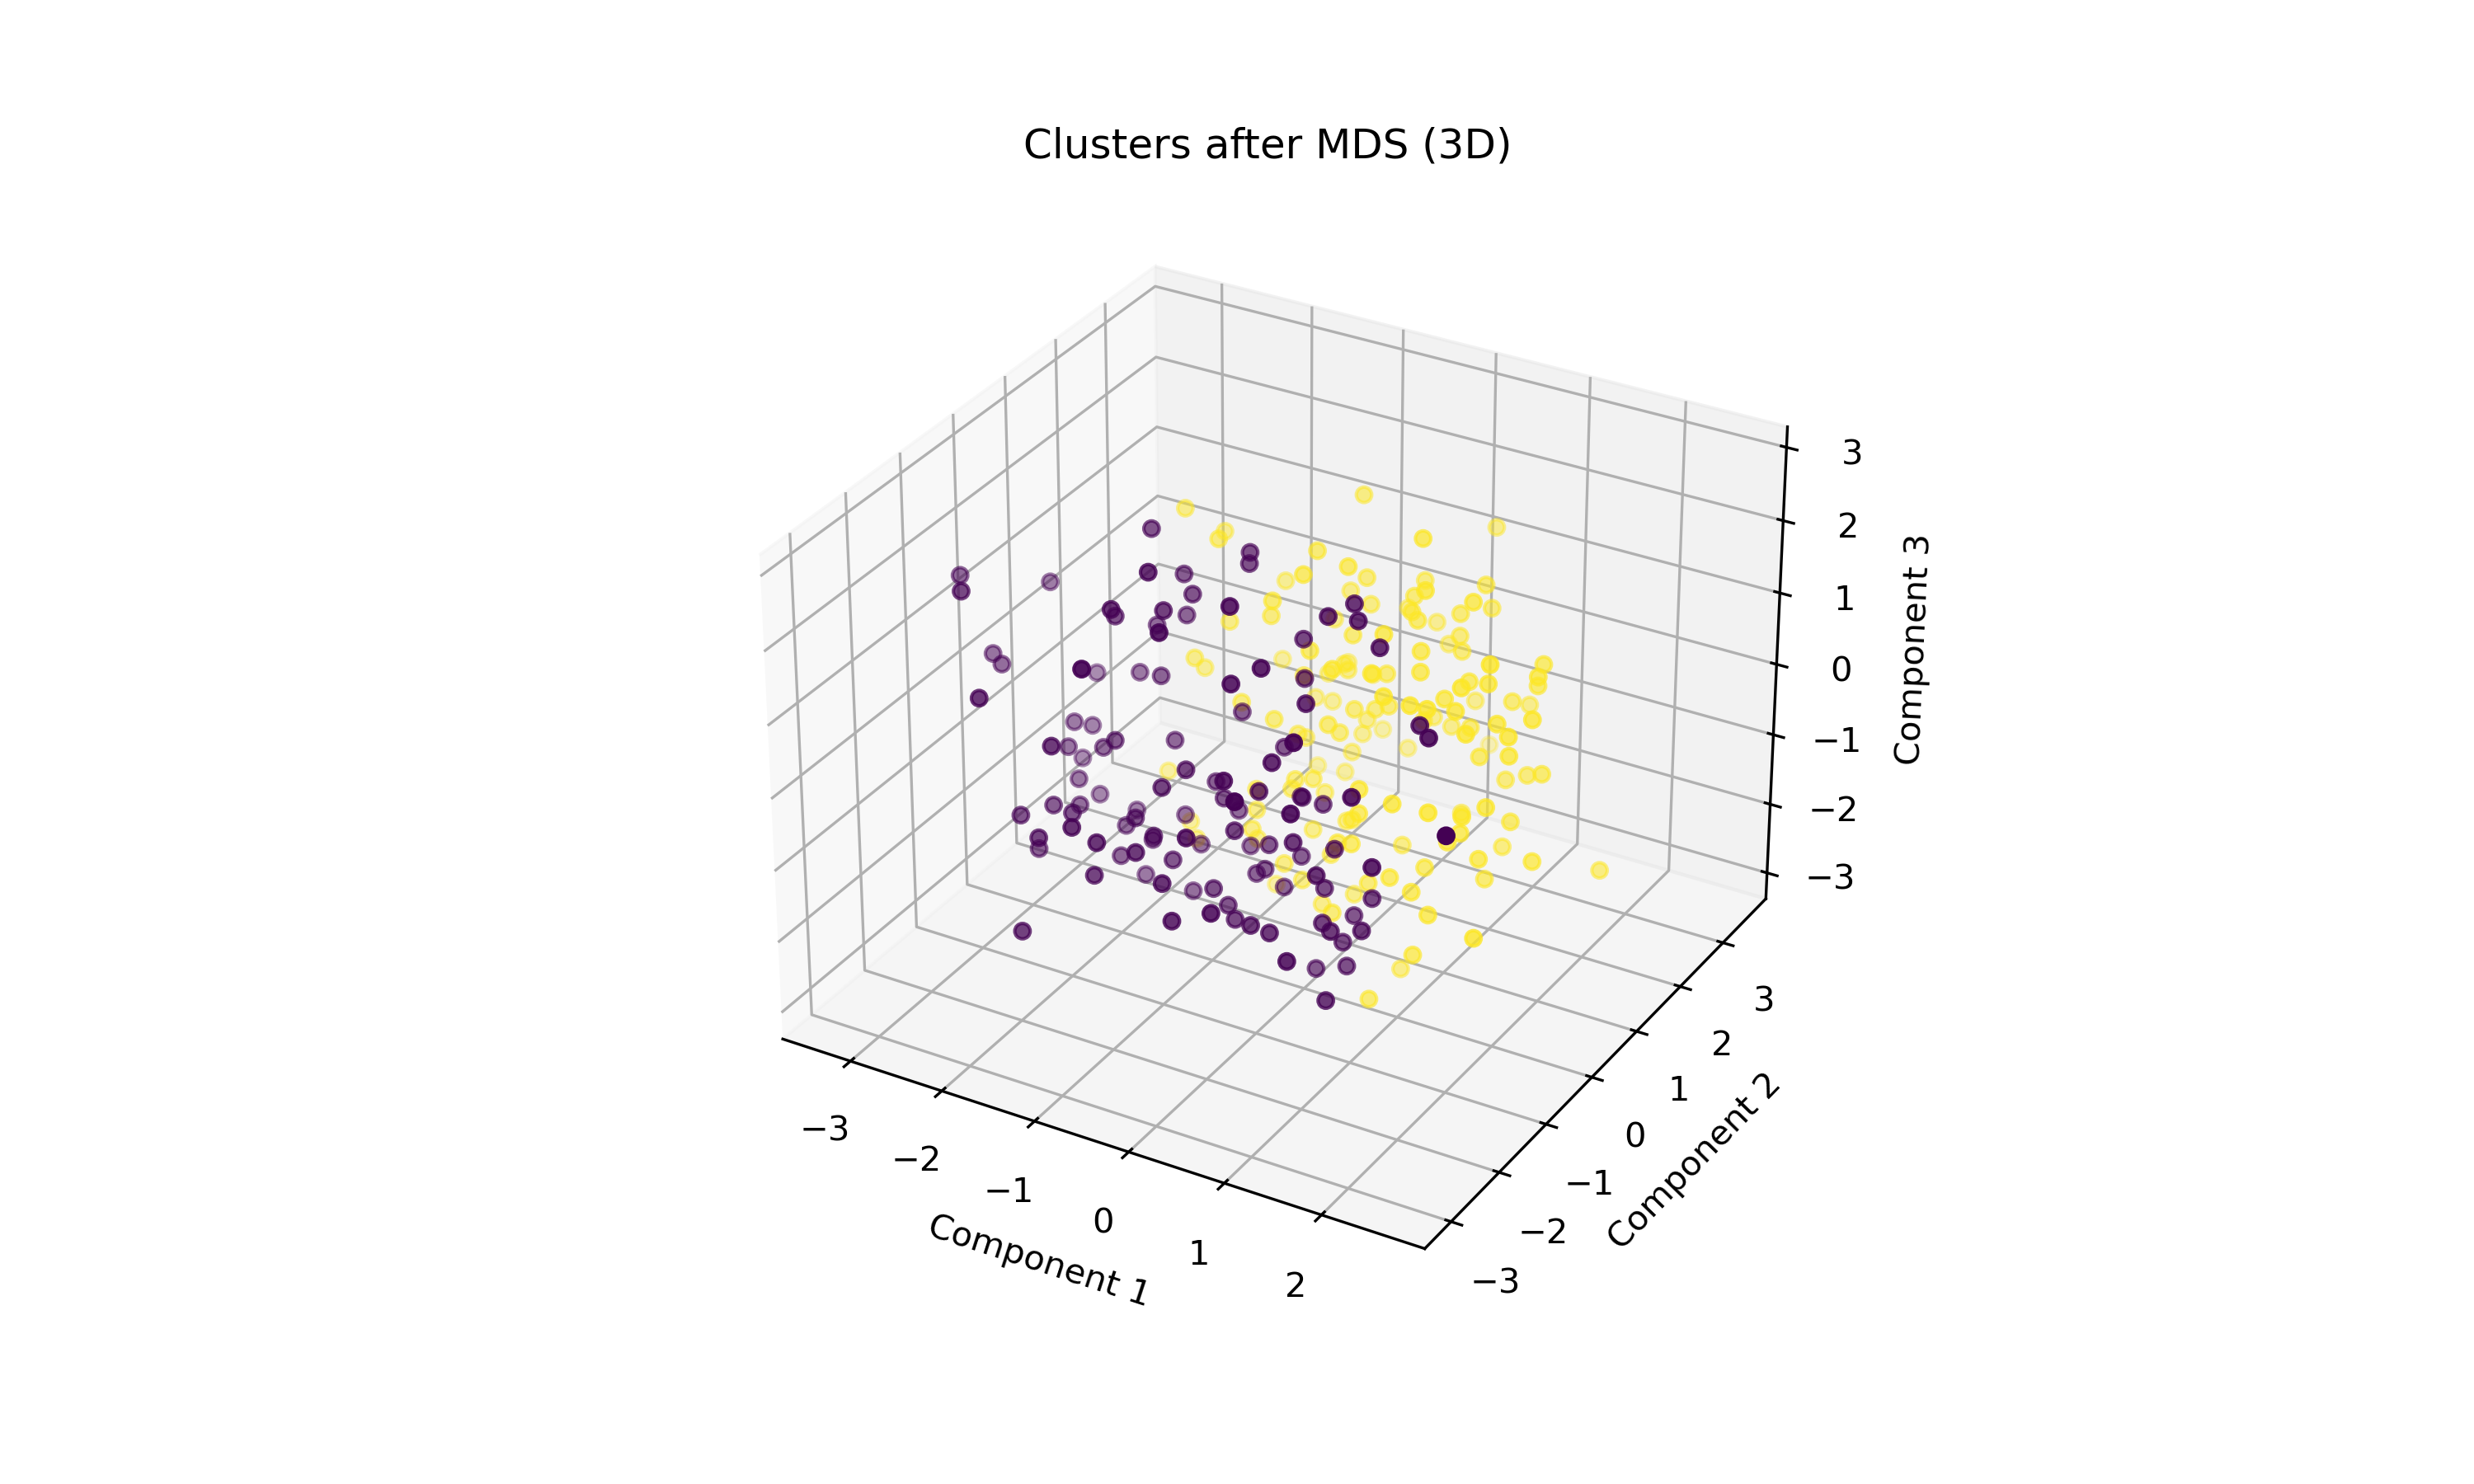
\includegraphics[width=0.5\linewidth]{MDS_3D.png}
    \caption{Clusters after MDS (3D)}
    \label{fig:mds_3d}
\end{figure}

\section{Conclusion}
The analysis of various nonlinear dimension reduction techniques reveals that:
\begin{itemize}
    \item Methods like PCA, TruncatedSVD, and Kernel PCA provide consistent results in both 2D and 3D dimensions, suggesting reliable clustering performance.
    \item Factor Analysis shows promise with lower inertia values, indicating potentially more concentrated clusters.
    \item t-SNE, while effective for visualizing high-dimensional data, tends to produce more dispersed clusters, as evidenced by its higher inertia values.
    \item MDS demonstrates moderate performance, providing a balance between linear and nonlinear mapping approaches.
\end{itemize}
Overall, the choice of dimensionality reduction method should consider the specific characteristics of the data and the desired clustering outcomes.

\end{document}
